\documentclass[12pt]{report}
\usepackage{xcolor, colortbl}
\usepackage{algorithm}
\usepackage[noend]{algpseudocode}
\usepackage{textcomp}
\usepackage{listings}
\usepackage{hyperref}
\usepackage{alltt}
\usepackage{tikz}
\usepackage{framed}
\usepackage{mdframed}
\usepackage{marvosym}
\usepackage{wasysym}
\usepackage{marvosym}
\usepackage{crayola}
\usepackage{mathpartir}
\usepackage{tabularx}
\usepackage[belowskip=-15pt,aboveskip=0pt]{caption}
\usepackage[skins]{tcolorbox}
\usepackage{multicol}
\usetikzlibrary{positioning,shapes,arrows, backgrounds, fit, shadows}
\usetikzlibrary{decorations.markings}
\usepackage{listings}
\usepackage[margin=1in]{geometry}
%\usepackage{mathptmx}
\usepackage{setspace}
\usepackage{natbib}
\usepackage{authblk}
\usepackage{enumitem}

\newcommand{\myheader}[1]{
	{\color{darkblue}
		\begin{Large}
			\begin{center}
				{#1}
			\end{center}
		\end{Large}
	}
}
\newcommand{\myminorheader}[1]{
	{\color{BrickRed}
		\begin{Large}
			{\fontfamily{\sfdefault}\selectfont\textbf{#1}}
		\end{Large}
	}
}

%\tikzstyle{input} = [coordinate]
%\tikzstyle{output} = [coordinate]


\tikzstyle{bb}=[%
      rectangle, draw=black, thick, fill=OliveGreen!30, drop shadow, align=center,
      text ragged, minimum height=2em, minimum width=2em, inner sep=6pt
]

\tikzstyle{inv}=[%
      rectangle, draw=none,  align=center,
      text ragged, minimum height=2em, minimum width=2em, inner sep=6pt
]

\tikzstyle{db}=[%
      ellipse, draw=black, thick, fill=pink, drop shadow, align=center,
      text ragged, minimum height=2em, inner sep=6pt
]

\tikzstyle{jn}=[%
      ellipse, draw=black, thick, fill=black, inner sep=0, outer sep=0,
]

\tikzstyle{io}=[%
      trapezium, trapezium left angle=60, trapezium right angle=120, draw=black, thick, fill=brown, drop shadow,
      text ragged, minimum height=2em, minimum width=2em, inner sep=6pt, align=center
]

\tikzstyle{glio}=[%
      trapezium, trapezium left angle=60, trapezium right angle=120, draw=red, line width = 1mm, fill=brown, drop shadow,
      text ragged, minimum height=2em, minimum width=2em, inner sep=6pt
]
\tikzstyle{gl}=[%
      rectangle, draw=red, line width = 1mm, fill=lightblue, drop shadow,
      text ragged, minimum height=2em, minimum width=2em, inner sep=6pt
]

\tikzstyle{en}=[%
      rectangle, draw=black, thick, fill=none,
      text ragged, minimum height=2em, minimum width=2em, inner sep=6pt
]

\tikzstyle{sh}=[%
      rectangle, draw=gray, thick, fill=none, color = gray,
      text ragged, minimum height=2em, minimum width=2em, inner sep=6pt
]


\lstdefinestyle{pc}{
	language = Python,
	basicstyle = \small\ttfamily,
	stringstyle = \ttfamily\color{Purple},
	keywordstyle=\color{black}\bfseries,
	identifierstyle=\ttfamily\color{BrickRed},
	frame=single,
	frameround=tttt,
	numbers=none,
	showstringspaces=false
}

\lstdefinestyle{cppc}{
	language = C++,
	basicstyle = \ttfamily\small,
	stringstyle = \color{red}\ttfamily,
	keywordstyle=\color{Blue}\bfseries,
	identifierstyle=\ttfamily,
	frame=single,
	frameround=tttt,
	numbers=none,
	showstringspaces=false,
	mathescape=true,
	escapeinside={(*@}{@*)}
}

\lstdefinestyle{occ}{
	language = Caml,
	basicstyle = \ttfamily,
	stringstyle = \color{red}\ttfamily,
	keywordstyle=\color{Blue}\bfseries,
	identifierstyle=\ttfamily,
	frameround=tttt,
	numbers=none,
	showstringspaces=false,
	mathescape=true,
	escapeinside={(*@}{@*)}
}

\lstdefinestyle{oc}{
	language = bash,
	backgroundcolor = \color{black!60},
	basicstyle = \ttfamily\color{white},
	stringstyle = \color{red}\ttfamily,
	keywordstyle=\color{white}\bfseries,
	identifierstyle=\ttfamily,
	frameround=tttt,
	numbers=none,
	showstringspaces=false,
	mathescape=true,
	escapeinside={(*@}{@*)}
}

\newcommand{\myslide}[1]{
\textbf{Slide:} \\
	\begin{framed}
			{#1}
	\end{framed}
}

\newcommand{\mynote}[1]{
\vspace{1cm}
\textbf{Note:} \\
	\fbox{
		\parbox{\textwidth}{%
			\colorbox{green!25}{
				\begin{minipage}{\textwidth}
					{#1}
				\end{minipage}
			}
		}
	}
}

\newcommand{\kctt}[1]{{\color{Red}{\lstinline[basicstyle=\ttfamily, mathescape=true]@#1@}}}

\title{A System for Automated Evaluation of Objective Questions}
\begin{document}


\chapter{User Manual}

\section{Basic Concepts}
\subsection{Quiz Type}
This software supports two types of objective question quizzes:
\begin{enumerate}
\item \textbf{Simple quiz:} In this quiz, the students are supposed to answer all questions. All students answer the same question paper.
\item \textbf{Jumbled quiz:} In this form of quiz, each student gets a different question paper to answer, which contains questions sampled out of a larger item bank and jumbled.
\end{enumerate}

\subsection{Question Types}
There are two types of questions that can be included in the question papers: multiple choice questions (MCQ) and match the following (MTF).
An MCQ is a question with two or more possible options out of which one or more may be correct choices. For example:

\begin{mdframed}
Name two dynamically typed programming languages:

\begin{enumerate}
\item Java
\item \label{i:py} \textbf{Python}
\item Haskell
\item \label{i:ru} \textbf{Ruby}
\end{enumerate}
\end{mdframed}

In the above, options \ref{i:py} and \ref{i:ru} are correct answers.

The second question type is match the following.

\begin{mdframed}
Match the following programming languages on the left column with properties on the right:

\begin{tabular}{c @{} c}
\begin{minipage}{0.4\textwidth}
\begin{enumerate}
\item Python
\item Java
\item C++
\item OCaml
\end{enumerate}
\end{minipage}
&
\begin{minipage}{0.4\textwidth}
\begin{enumerate}[label=\Alph*.]
\item \label{i:st} Static typing
\item \label{i:dt} Dynamic typing
\item \label{i:ut} Untyped
\item \label{i:it} Implicit typing
\item \label{i:et} Explicit typing
\item \label{i:func} Functional
\item \label{i:oo} Object oriented
\end{enumerate}
\end{minipage}
\end{tabular}
\end{mdframed}

In the above example, the matches are as follows
\begin{enumerate}
\item Python matches with \ref{i:dt}, \ref{i:it}, \ref{i:func} and \ref{i:oo}
\item Java match with \ref{i:st}, \ref{i:et} and \ref{i:oo}
\item C++ match with \ref{i:st}, \ref{i:et} and \ref{i:oo}
\item OCaml match with \ref{i:st}, \ref{i:it}, \ref{i:func},  and \ref{i:oo}
\end{enumerate}

A few points to note here:
\begin{itemize}
\item The mapping can be many to many, even allowing some options on the either side to have no matches at all (e.g. \ref{i:ut}).
\item There is no restriction on the number of options on either columns. For example, in the above example, we have 4 options on the LHS and 7 on the RHS.
\end{itemize}


\section{Simple Quiz}

\begin{figure}[H]
\begin{center}
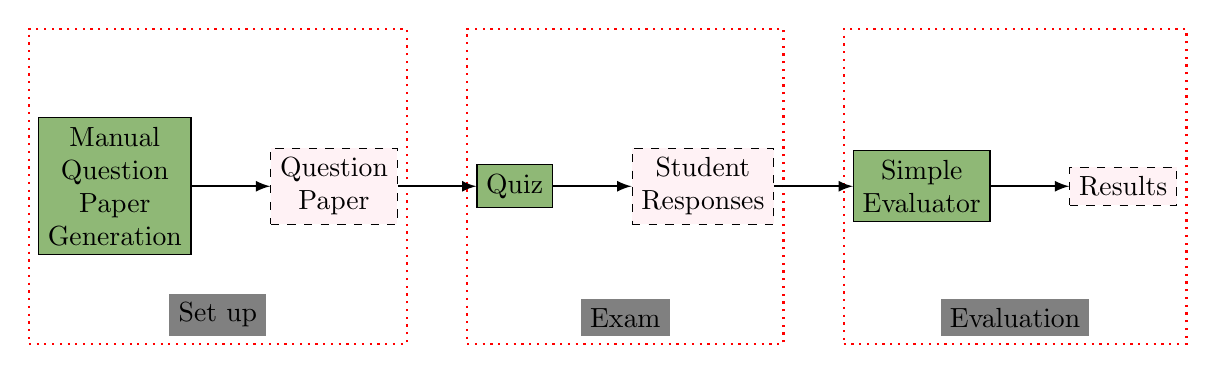
\begin{tikzpicture}
\node[draw=Black, fill=OliveGreen!50, align=center](qpgen){Manual \\ Question \\ Paper \\ Generation};
\node[dashed, draw=Black, fill=Pink!20, align=center, right=of qpgen](qp){Question \\ Paper};
\node[draw=Black, fill=OliveGreen!50, align=center, right=of qp](quiz){Quiz};
\node[dashed, draw=Black, fill=Pink!20, align=center, right=of quiz](sresp){Student \\ Responses};
\node[draw=Black, fill=OliveGreen!50, align=center, right=of sresp](seval){Simple \\ Evaluator};
\node[dashed, draw=Black, fill=Pink!20, align=center, right=of seval](res){Results};

\node[draw=Red, dotted, thick, minimum height=4cm, fit = (qpgen) (qp)] (setup) {};
\node[fill=Gray, above=0.1cm of setup.south](lsetup){Set up};

\node[draw=Red, dotted, thick, minimum height=4cm, fit = (quiz) (sresp)] (exam) {};
\node[fill=Gray, above=0.1cm of exam.south](lexam){Exam};

\node[draw=Red, dotted, thick, minimum height=4cm, fit = (res) (seval)] (eval) {};
\node[fill=Gray, above=0.1cm of eval.south](eval){Evaluation};

\draw[-latex, thick] (qpgen) -- (qp);
\draw[-latex, thick] (qp) -- (quiz);
\draw[-latex, thick] (quiz) -- (sresp);
\draw[-latex, thick] (sresp) -- (seval);
\draw[-latex, thick] (seval) -- (res);

\end{tikzpicture}
\end{center}
\caption{Simple Quiz Workflow}
\label{f:squiz}
\end{figure}
The question paper creation for a simple quiz is manual. All students solve an identical question paper. The evaluation step directly runs on the student responses using the \lstinline[style=pc]@SimpleEvaluator@ module.

\subsection{Setup}
Suppose you intend to conduct a simple quiz. As mentioned above, in a simple quiz, all students solve the same question paper. Such a quiz is ideal when there is small class and enough assurance that cheating is not a possibility. Of course, all questions are assumed to be either multiple choice questions (MCQ) or match the following questions (MTF).


The assessment project can be setup conveniently using the setup utility. The setup utility automatically generates the skeletal infrastructure for conducting such a quiz.

\section{Jumbled Quiz}
\begin{figure}[H]
\begin{center}
\resizebox{\textwidth}{!}{
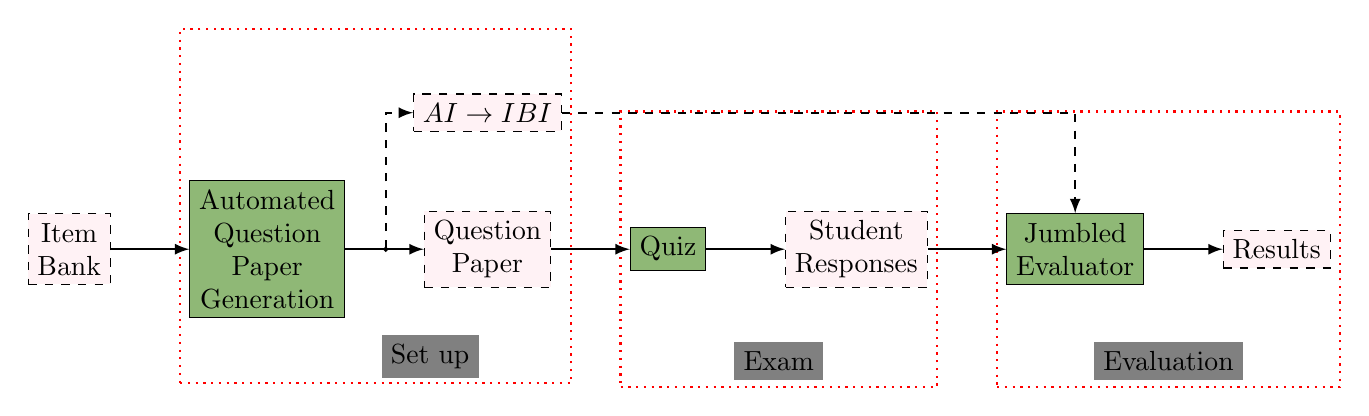
\begin{tikzpicture}
\node[dashed, draw=Black, fill=Pink!20, align=center](ib){Item \\ Bank};
\node[draw=Black, fill=OliveGreen!50, align=center, right=of ib](qpgen){Automated \\ Question \\ Paper \\ Generation};

\node[jn, right=0.5cm of qpgen](jn1) {};
\node[dashed, draw=Black, fill=Pink!20, align=center, right=of qpgen](qp){Question \\ Paper};
\node[dashed, draw=Black, fill=Pink!20, align=center, above=of qp](aiibi){$AI\rightarrow IBI$};

\node[draw=Black, fill=OliveGreen!50, align=center, right=of qp](quiz){Quiz};
\node[dashed, draw=Black, fill=Pink!20, align=center, right=of quiz](sresp){Student \\ Responses};
\node[draw=Black, fill=OliveGreen!50, align=center, right=of sresp](jeval){Jumbled \\ Evaluator};
\node[dashed, draw=Black, fill=Pink!20, align=center, right=of jeval](res){Results};

\node[draw=Red, dotted, thick, minimum height=4.5cm, fit = (qpgen) (qp) (aiibi)] (setup) {};
\node[fill=Gray, above right=0.1cm of setup.south](lsetup){Set up};

\node[draw=Red, dotted, thick, minimum height=3.5cm, fit = (quiz) (sresp)] (exam) {};
\node[fill=Gray, above=0.1cm of exam.south](lexam){Exam};

\node[draw=Red, dotted, thick, minimum height=3.5cm, fit = (res) (jeval)] (eval) {};
\node[fill=Gray, above=0.1cm of eval.south](eval){Evaluation};

\draw[-latex, thick] (ib) -- (qpgen);
\draw[-, thick] (qpgen) -- (jn1);

\draw[-latex, thick] (jn1) -- (qp);
\draw[-latex, dashed, thick] (jn1) |- (aiibi);

\draw[-latex, thick] (qp) -- (quiz);
\draw[-latex, thick] (quiz) -- (sresp);
\draw[-latex, thick] (sresp) -- (jeval);
\draw[-latex, dashed, thick] (aiibi) -| (jeval);

\draw[-latex, thick] (jeval) -- (res);

\end{tikzpicture}
}
\end{center}
\caption{Jumbled Quiz Workflow}
\label{f:jquiz}
\end{figure}

The question paper creation step uses the \kctt{genAIs} (generate assessment items) module. Once the question papers are generated, quiz is conducted. Finally, the automated evaluation process takes place using the \lstinline[style=pc]@JumbledEvaluator@ module.

As you would have observed, the workflow for jumbled quiz remains the same at high level as that of simple quiz. The difference lies in the fact that a separate question paper is generated for each roll number. This mapping is maintained in $AI\rightarrow IBI$ data item by the system. Note that $AI\rightarrow IBI$ doesn't concern the user. It is an internal artifact of the system (and hence shown connected through dashed lines to the rest of the system in Figure~\ref{f:jquiz}) and is later used by the evaluator to map back the questions to their source in the item bank for evaluation purpose.
\section{Getting Started with a Demo}
Let's get a bit hands on by running a demo and feeling our way around with the system. We assume that you would be using a bash like command shell for interacting with the system. We call the evalobj directory as \kctt{APPHOME}.
\subsection{Start the demo}

Go to the demo directory:
\begin{lstlisting}[style=oc]
cd APPHOME/test/j2/quizzes/demo
\end{lstlisting}


Clean up the directory:
\begin{lstlisting}[style=oc]
./reset.sh
\end{lstlisting}

Take a look at the contents of the directory.
\begin{lstlisting}[style=oc]
backup  config.json  packages  __pycache__  reset.sh
\end{lstlisting}

The only file here which is important to notice is the configuration file \kctt{config.json}. Every quiz will have its own configuration file with all the relevant meta-data pertaining to the quiz.

Its contents (as they stand on date)are reproduced here:

\lstinputlisting[basicstyle=\ttfamily\scriptsize, frame=single]{../test/j2/quizzes/demo/config.json}

Here are the important fields of the configuration file and their meanings:
\begin{itemize}
\item \kctt{course name}: Name of the course
\item \kctt{course code}: Course code as prescribed by the university
\item \kctt{assessment name}: The exam name. Here it's ``demo", but in practice it could something like ``Quiz 1", ``Mid-term Examination" etc.
\item \kctt{assessment type}: This is the quiz type. Currently, there are two types available: \kctt{simple} and \kctt{jumbled}.
\item \kctt{roll number file}: The full path of the file which contains the roll numbers of all the students taking the examination. Note that the roll number file needs to have the roll numbers in a particular way. As it stands today, the required format is that the roll numbers will be listed in column 1 of a CSV file starting with the second row, the first row having the header ``Roll Number". For example:
\lstinputlisting[basicstyle=\ttfamily\scriptsize, frame=single]{../test/j2/class.csv}
\item \kctt{assessment home}: This directory -- for the application to know during runtime.
\item \kctt{number of items per assessment instrument}: Number of questions you want on your question paper. Its relevance is based on the quiz type. In particular, a jumbled quiz will generate question papers each having so many questions on it. Simple quiz will simply ignore this field.
\item \kctt{items}: This is the list of questions in the item bank. Here, we list 4 items named \kctt{item1}, \kctt{item2}, \kctt{item3} and \kctt{item4}. Each is an MCQ with 4 options and carrying 1 mark.  
\end{itemize}

Note that everytime we are creating a new quiz, config.json has to be created. Smooth flow of the rest of the process would depend on our writing this file properly.

\subsection{Generate the quiz}

\begin{lstlisting}[style=oc]
APPHOME/src/setup.py config.json
\end{lstlisting}

This generates all the necessary files for the quiz. Let's take a look at the contents of the directory:
\begin{lstlisting}[style=oc]
assessment-instruments  backup  config.json  config.py  evaluation  gen.py  item-bank  packages  __pycache__  reset.sh
\end{lstlisting}
\begin{itemize}
\item \kctt{assessment-instruments}: This is the directory created -- currently empty -- to contain the question papers once they are generated.
\item \kctt{config.py}: This is the file which contains the Python translation of the contents of the \kctt{config.json} file.
\item \kctt{evaluation}: This is the evaluation directory. The \kctt{evaluate.py} file is the evaluator file which will be run once the quiz is conducted and submissions have come in.
\item \kctt{gen.py}: This script needs to be run next to generate the quiz.
\item \kctt{item-bank}: This contains the item bank, in the form of stubs of \LaTeX\ text. These need to be filled up create the question papers. Note that there are five item stubs created, since that's the number of items mentioned in \kctt{config.json}. For example, the contents of the item1.tex is:
\begin{lstlisting}[basicstyle=\ttfamily\small, frame=single]
\question
\label{q:SE101:demo:item1}
\begin{enumerate}
	\item option 1
	\item option 2
	\item option 3
	\item option 4
\end{enumerate}

\end{lstlisting}
\item \kctt{packages}: When the \kctt{gen.py} file is executed, it is this directory -- currently empty -- where the question papers will be generated. 
\end{itemize}

\subsection{Generate the Question Papers}
Run the \kctt{gen.py} script.
\begin{lstlisting}[style=oc]
python3 gen.py
\end{lstlisting}
The main effect of running this script would that the \kctt{packages} directory is no more empty. It contains one directory for each roll number. In there, among other files, you will find the question paper for that roll number: \kctt{packages/rn1/rn1.pdf}, \kctt{packages/rn2/rn2.pdf}, \kctt{packages/rn3/rn3.pdf} and \kctt{packages/rn4/rn4.pdf}.

There's one more change, though it needn't concern the user: a new file \kctt{AItoIBI.csv} has been generated. It's the mapping from roll assessment instrument to item bank items. As I type this, it looks like the following:

\begin{center}
\begin{tabular}{|c|c|c|c|}
\hline
\kctt{rn2}&\kctt{item5}&\kctt{item3}&\kctt{item4} \\
\hline
\kctt{rn3}&\kctt{item4}&\kctt{item1}&\kctt{item3} \\
\hline
\kctt{rn4}&\kctt{item4}&\kctt{item3}&\kctt{item2} \\
\hline
\kctt{rn1}&\kctt{item2}&\kctt{item4}&\kctt{item1} \\
\hline
\end{tabular}
\end{center}

Again, it's not important for the user to know how to read it. However, for the curious minded, it means the following:
Each row provides the source of each question in an assessment instrument (question paper). For example, for the assessment instrument \kctt{rn2} (first row), the first item is \kctt{item5} of the item bank, the second item is \kctt{item3} of the item bank and the third item is \kctt{item4} of the item bank.

This completes the process of generating the question papers.

\subsection{Administer the Quiz}
At the time of administering the quiz, these question papers can be shared with the students using an appropriate external method, e.g. email, LMS or a shared drive. This is outside the purview of this system.

At the end of administering the quiz, the submitted answers are provided in the submissions directory in a particular format. In this demo, we simulate the process of answer submission by running the backup script provided.

\begin{lstlisting}[style=oc]
cd backup
./restore.sh
cd ..
\end{lstlisting}

Once this is done, a new directory named submissions is created. Let's examine the contents of the submissions directory. You find the following contents:

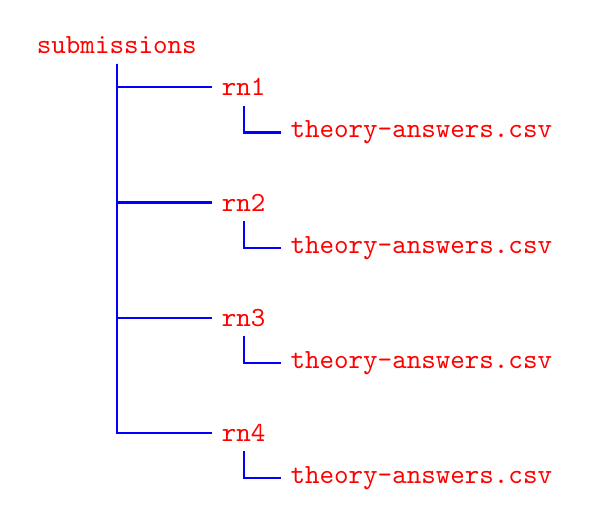
\begin{tikzpicture}
\node(submissions) {\kctt{submissions}};
\node(rn1) [below right=0.1cm of submissions]{\kctt{rn1}};
\node(ta1) [below right=0.1cm of rn1]{\kctt{theory-answers.csv}};
\node(rn2) [below =1cm of rn1]{\kctt{rn2}};
\node(ta2) [below right=0.1cm of rn2]{\kctt{theory-answers.csv}};
\node(rn3) [below =1cm of rn2]{\kctt{rn3}};
\node(ta3) [below right=0.1cm of rn3]{\kctt{theory-answers.csv}};
\node(rn4) [below =1cm of rn3]{\kctt{rn4}};
\node(ta4) [below right=0.1cm of rn4]{\kctt{theory-answers.csv}};

\draw[-, thick, Blue] (submissions) |- (rn1);
\draw[-, thick, Blue] (submissions) |- (rn2);
\draw[-, thick, Blue] (submissions) |- (rn3);
\draw[-, thick, Blue] (submissions) |- (rn4);
\draw[-, thick, Blue] (rn1) |- (ta1);
\draw[-, thick, Blue] (rn2) |- (ta2);
\draw[-, thick, Blue] (rn3) |- (ta3);
\draw[-, thick, Blue] (rn4) |- (ta4);
\end{tikzpicture}

Each CSV file \kctt{submissions/rn$i$/theory-answers.csv} is the answer sheet of \kctt{rn$i$}. 

Another effect of this step is a bit of a cheating! It over-writes the \kctt{AItoIBI.csv file} to ensure that the answers in the submitted answer sheets match the item bank items properly\footnote{Note that the question paper to item bank items mapping was generated randomly. Hence, it is impossible to reproduce using an already stored set of answers.}. However, if this seems confusing at this point, please simply ignore it.

The final effect of this step is addition of a new file \kctt{theory-answers.csv} in the \kctt{evaluation} directory. This file corresponds to the instructor's reference solution. Its contents are as follows:
\begin{center}
\begin{tabular}{|c|c|c|c|}
\hline
1 & & & \\
\hline
1 & 2 & & \\
\hline
3 & & & \\
\hline
3 & 4 & & \\
\hline
1 & 2 & 3 & 4 \\
\hline
\end{tabular}
\end{center}

\subsection{Evaluate the Quiz}
To evaluate the quiz, simply enter the evaluation directory and run the evaluate script:
\begin{lstlisting}[style=oc]
cd evaluation
python3 evaluate.py
\end{lstlisting}

You will see the following output:
\begin{lstlisting}[style=oc]
evaluating  rn1  ...
evaluating  rn2  ...
evaluating  rn3  ...
evaluating  rn4  ...
rn3 	 3.0
rn1 	 3.0
rn4 	 3.0
rn2 	 3.0
total marks =  roll number: reference
item scores: [1.0, 1.0, 1.0, 1.0, 1.0]
total score: 5.0
\end{lstlisting}

The result of evaluation is stored in the \kctt{result.csv} file in the \kctt{evaluation} directory. As of now, it looks like the following:
\begin{center}
\begin{tabular}{|c|c|c|c|c|c|c|}
\hline
rn3 & 1.0 & 0 & 1.0 & 1.0 & 0 & 3.0 \\
\hline
rn1 & 0 & 0 & 1.0 & 1.0 & 1.0 & 3.0 \\
\hline
rn4 & 1.0 & 0 & 1.0 & 1.0 & 0 & 3.0 \\
\hline
rn2 & 1.0 & 1.0 & 0 & 0 & 1.0 & 3.0 \\
\hline
\end{tabular}
\end{center}

This tabulates the marks each roll number (row) has got for each question (column). For example, the first row says that \kctt{rn3} has scored \kctt{1.0} for \kctt{item1}, \kctt{0} for \kctt{item2}, \kctt{1.0} for \kctt{item3}, \kctt{1.0} for \kctt{item4} and \kctt{0} for \kctt{item5}. The total score for \kctt{rn3} is \kctt{3} as summarised in column 7. Note that the items for which \kctt{rn3} has score 0 (i.e. \kctt{item2} and \kctt{item4}) are those which were not there in its question paper, which means the student scored full-marks.


\chapter{Design}
\section{Question Paper Codes}

\subsection{Question Paper Generation}
To discourage cheating in the class, we generate a set of question papers by randomly selecting $n$ questions out of an item-bank of $N$ questions. A set $K$ of distinct \emph{assessment instruments} are generated, numbered 0, 1, ..., $|K-1|$. We call them \emph{assessment instruments}.

The \emph{question paper generator} module $G$ generates a set $C$ of codes each of which can be mapped to any one of the assessment instruments of $K$. Each of the code $c$ in $C$ is finally mapped to one distinct question paper with $c$ printed on it. This way, the students will not be able to identify which assessment instrument $k \in K$ their copy of the question paper belongs to. Each question paper will have an empty table called the \emph{response table} on page one which will be used by the student to fill in his responses.

$G$ also generates a map from assessment instrument to question order. This tells us the original question number of each item in the give assessment instrument. For example:
\begin{figure}

\begin{center}
\begin{tabular}{|c|c|c|c|c|c|c|c|c|c|c|}
\hline
\cellcolor{Gray}0 & 3 & 5 & 1 & 4 & 9 & 12 & 15 & 2 & 10 & 2 \\
\hline
\cellcolor{Gray}1 & 4 & 1 & 2 & 11 & 6 & 7 & 5 & 14 & 8 & 12 \\
\hline
& \multicolumn{10}{|c|}{...} \\
\hline
\cellcolor{Gray}9 & 5 & 12 & 2 & 1 & 6 & 7 & 3 & 11 & 8 & 10 \\
\hline
\end{tabular}
\end{center}

\caption{Assessment Instrument Item to Item Bank Item map $AII \mapsto IBI$}
\label{f:aiiibi} 
\end{figure}

Figure~\ref{f:aiiibi} shows a possible mapping from assessment instruments to item bank items. The table can be interpreted as follows: There are 10 assessment instruments numbered 0 through 9. For each assessment instrument $AI \in K$ (here $|K| = 10$), there is a row in the table. Each cell in that row has the item bank item number for that item. For instance, for $AI = K[0]$, $AI[0] = 3$, $AI[1] = 5$ and so on.
  
This module will generate a map -- called $QP\mapsto AI$ between \emph{question paper code} to \emph{assessment instrument}. For example:

$QP\mapsto AI = [0, 1, 2, ..., 9, 0, 1, 2, ...]$ could be one such mapping. It says that $QP\mapsto AI[0] = 0$ (i.e. the question paper with code $0$ maps to assessment instrument number $0$). Similarly, $QP\mapsto AI[11] = 1$ (i.e. the question paper with code $11$ maps to assessment instrument number $1$) and so on.

\subsection{TA's Job}
The TA will note down following:
\begin{enumerate}
\item Question paper code for each roll number creating a \emph{roll number} to \emph{question paper code} map $RN\mapsto QP$.
\item transfer the responses into a CSV file corresponding to each student exactly as in the response table.
\end{enumerate}

\subsection{Automated Evaluation}
The \emph{response rearranger} refers to the $RN\mapsto QP$ and $QP\mapsto AI$ map to extract the assessment instrument for each roll number. Using this, the evaluator rearranges the responses in the order as per the item bank to create a rearranged response for the roll number $n$, $R'(n)$. This is given to the evaluator for final automated evaluation.
\end{document}
